\chapter{EU-Beitritt als Option}
Seit dem Ende der kriegerischen Auseinandersetzungen auf dem Balkan in den 1990er Jahren in Folge des Auseinanderbrechens Jugoslawiens besteht für die Länder des Westlichen Balkans \footnote{Kroatien, Serbien, Montenegro und Mazedonien, Albanien, Bosnien-Herzegowina, Kosovo.}  die Option für einen Beitritt zur EU. Allen Staaten des Westlichen Balkans wurde im Juni 2003 vom Europäischen Rat in Thessaloniki eine konkrete EU-Beitrittsperspektive eröffnet. Mazedonien\footnote{Aufgrund eines Namensstreites mit Griechenland ist der offizielle Name „Former Yugoslav Republic of Macedonia“ (FYROM), unter dem das Land 1993 in die Vereinten Nationen aufgenommen wurde. Für einen besseren Lesefluss wird in der vorliegenden Arbeit die Bezeichnung Mazedonien verwendet.}, Montenegro und Serbien haben inzwischen die Stufe von Beitrittskandidaten erreicht, während Albanien, Bosnien-Herzegowina und Kosovo potenzielle Beitrittskandidaten sind. Slowenien, auch ein Nachfolgestaat Jugoslawiens, war schon in der letzten Aufnahmewelle 2004 zusammen mit Ländern Osteuropas in die EU aufgenommen worden, Kroatien ist am 1. Juli 2013 in die EU aufgenommen worden.\par

Der Westbalkan ist von EU-Mitgliedern umgeben (Ungarn, Griechenland, Slowenien, Bulgarien, Italien, Slowakei). So gesehen handelt es sich bei den noch nicht beigetretenen Ländern des Westbalkans quasi um einen „weißen Fleck“ mitten in Europa. Vor dem Hintergrund der fragilen Situation auf dem Balkan nach der Auflösung Jugoslawiens und der potenziell instabilen staatlichen Gebilde (Bosnien-Herzegowina, Kosovo) erscheint eine konkrete EU-Perspektive nachvollziehbar.\par

Für die Europäische Union ist das Bestehen dieses „weißen Fleckes“ ein Problem, für das Lösungen gesucht wurden. Eine anscheinend sinnvolle Lösung ist die erneute Erweiterung der EU mittels der Integration der Länder des Westbalkans. Das Interesse der EU ist dabei auch ein strategisches, nicht zuletzt zur Vermeidung eines Konfliktherdes „vor der Haustüre“. Dieses strategische Interesse schließt gleichzeitig die Hoffnung auf einen Reformmotor mit ein, wie es auch in der folgenden Äußerung Javier Solanas\footnote{Generalsekretär des Rates der Europäischen Union von 1999 bis 2009 und in dieser Zeit Hoher Vertreter für die Gemeinsame Außen- und Sicherheitspolitik (GASP).} zum Ausdruck kommt:\par

„It is in the European interest that countries on our borders are well governed. Neighbours who are engaged in violent conflict, weak states where organised crime flourishes, dysfunctional societies or exploding population growth on its borders all pose problems for Europe. […] The credibility of our foreign policy also depends on the successes achieved in the region. The European perspective is both a strategic goal and an incentive for reform” \cite{solana}.\par

In den Staaten des Westbalkans selbst ist die Aufnahme in die Europäische Union ein vorrangiges Ziel. Damit verbunden sind Hoffnungen auf ein vor allem ökonomisch schnelleres Heranrücken an europäische (Lebens-)Standards.\par

Im Prozess der Ausrichtung der neu entstandenen Westbalkanstaaten auf demokratische Werte und Marktwirtschaft spielten internationale Organisationen seit Anfang der 1990er Jahre eine wesentliche Rolle als Unterstützer sowohl finanzieller Art als auch mit Beratungsleistungen. Im Westbalkan waren dies vor allem das United Nations Development Programm (UNDP), die US-amerikanische Entwicklungshilfeorganisation USAID, die Organisation für Sicherheit und Zusammenarbeit in Europa (OSZE) und die Weltbank sowie die Einrichtung eines Stabilitätspaktes für den Westbalkan (1999). Die EU mit ihrer Agency for Reconstruction (EAR), die in Kosovo, Serbien, Montenegro und Mazedonien die EU-Hilfe koordinierte, kam Ende 2002 hinzu. Ursprünglich war die Hilfe für die neu entstandenen Staaten des Westbalkans auf strukturelle Hilfen und Entwicklungshilfe ausgelegt. Mit zunehmendem Engagement der EU in der Region und nach dem EU-Gipfel von Thessaloniki von 2003 wurde den Ländern des Westlichen Balkans die konkrete EU-Perspektive eröffnet. In der Folge legte die EU für die Region ein Instrumentarium auf, das gezielte EU-Unterstützung im Vorfeld einer möglichen EU-Mitgliedschaft beinhaltete. Die Staaten des Westbalkans werden von der EU als Beitrittskandidaten oder potenzielle Beitrittskandidaten \footnote{Der Statuswechsel von potenziellem Beitrittskandidaten zum Beitrittskandidaten wird vom Rat der EU auf Grundlage einer Stellungnahme der Europäischen Kommission einstimmig entschieden.} durch Programme der pre-accessioning assistance in erheblichem Maße finanziell unterstützt. Diese Instrumente sollen ihnen die Heranführung an Standards ermöglichen, die Voraussetzung für die Aufnahme in die EU sind. Die Unterstützung bezieht sich im Rahmen des Institutionenaufbaus explizit auch auf die Reform der öffentlichen Verwaltung.
\section{Untersuchungsgegenstand}
Für eine Aufnahme in die EU müssen alle zukünftigen Mitgliedstaaten bestimmte Bedingungen erfüllen. Dabei geht es im Wesentlichen um die Annäherung an europäische Standards im Bereich Wirtschaft, Institutionenaufbau und Rechtsstaatlichkeit. Für die erfolgreiche Umsetzung einer Annäherung an die EU muss der gesamte gemeinsame Besitzstand (Acquis communautaire) übernommen werden. Das heißt, die Länder müssen ca. 100.000 Seiten gemeinschaftliche gesetzliche Normen in ihr nationales Recht übernehmen.
Für einen so umfangreichen Prozess, die Übernahme der Europäischen Gesetzgebung in nationales Recht, ist eine effektive öffentliche Verwaltung notwendig.\par
Dennoch ist die Ausgestaltung der öffentlichen Verwaltung im Rahmen des Annäherungsmechanismus kein vorrangiges Thema im Erweiterungsprozess. In den jährlichen Fortschrittsberichten\footnote{Die Fortschrittsberichte der EU werden von der EU-Kommission jährlich im Spätherbst für jedes der Länder erstellt, die einen Beitrittsantrag zur EU gestellt haben. In diesen Berichten wird aus Sicht der EU der Fortschritt des jeweiligen Landes zu den Themen der Kapitel des Acquis communautaire beschrieben.} der EU wird die öffentliche Verwaltung zwar regelmäßig thematisiert, allerdings nur unter politischen Gesichtspunkten. Als wesentlicher Grund hierfür kann gelten, dass der öffentlichen Verwaltung kein eigenes Kapitel im Acquis communautaire zukommt.\par
Im Rahmen der von der EU konzipierten Heranführungshilfe wird (finanzielle) Förderung bereitgestellt, um die Kandidatenländer für die EU „fit“ zu machen. Im Rahmen dieser Heranführungshilfe ist auch die Förderung einer effektiven öffentlichen Verwaltung der Länder im Blick. Der Umfang der finanziellen Förderung für die öffentliche Verwaltung in den Beitrittskandidaten ist allerdings nicht zu vergleichen mit der Förderung von solchen Themen, die im Acquis klar geregelt sind.\par
Es handelt sich gewissermaßen um eine paradoxe Situation. Einerseits ist die öffentliche Verwaltung essenziell wichtig für die erfolgreiche Heranführung von Beitrittskandidaten, andererseits scheint das Thema nicht im Zentrum des EU-Interesses zu stehen.\par
In der vorliegenden Arbeit wird dieser Zusammenhang in den Blick genommen. Die Entwicklung der öffentlichen Verwaltung in drei ausgewählten Ländern des Westlichen Balkans wird von verschiedenen Perspektiven aus betrachtet. Hauptbezugspunkt ist dabei die EU-Perspektive der Westbalkanstaaten in ihrer Bedeutung für die öffentliche Verwaltung.\par
Die Länder des Westlichen Balkans befinden sich mit der EU quasi in einem Verhandlungsprozess. Den Westbalkanländern wird die Mitgliedschaft in der EU in Aussicht gestellt, sie müssen dafür aber bestimmte Bedingungen erfüllen (Konditionalität). Dies ist ein intensiver, wechselseitiger Prozess der Annäherung seitens der Länder, welche die Mitgliedschaft anstreben und seitens der EU, die deren Bemühungen beobachtet, unterstützt und bewertet. \par
Die vorliegende Arbeit untersucht das Verhältnis zwischen den Ländern des Westlichen Balkans und der EU unter dem Gesichtspunkt der öffentlichen Verwaltung. Wichtig ist in diesem Zusammenhang die Darstellung des Status quo der öffentlichen Verwaltung in den drei Untersuchungsländern. Neben der Entwicklung seit der Demokratisierung wird auch die historische Entwicklung der öffentlichen Verwaltung in diesen drei Ländern näher beleuchtet und gefragt, wieweit frühere Zusammenhänge und Entwicklungen in die Gegenwart hinein wirken.\par
Die Untersuchung erfolgt im Wesentlichen auf zwei Ebenen.
\begin{itemize}
\item Die Theorie und Praxis der EU-Erweiterung mit der öffentlichen Verwaltung als Bezugspunkt.
\item Die vergleichende Perspektive am Beispiel der Verwaltungsentwicklung in drei benachbarten Westbalkanländern.
\end{itemize}
Die Kriterien für demokratische und verantwortungsvolle Regierungsführung haben sich international in den beiden letzten Dekaden verändert. Nicht mehr nur formale Parameter wie freie und faire Wahlen, Gewaltenteilung oder Rechtsstaatlichkeit stehen im Fokus der Betrachtung. Zunehmend wird nach „substantive democracy“ gefragt und damit eher outcome-orientierte Kriterien wie Institutionenentwicklung und die Wirkung von „Good Governance“ herangezogen (vgl. \cite{pridham99}). Die Perspektive der europäischen Integration ist dabei ein bestimmendes Moment, denn stabile Regierungspraxis und funktionsfähige Verwaltungsstrukturen sind Voraussetzungen für den Beitritt zur EU und die Übernahme des gemeinschaftlichen Besitzstandes (vgl. \cite{kemmeu}: 49).
\section{Untersuchungsziel}
Ziel der Untersuchung ist eine verwaltungswissenschaftliche Perspektive auf ein bisher eher politikwissenschaftlich bearbeitetes Thema: Die Erweiterung der EU nach Südosteuropa. Eine dezidiert verwaltungswissenschaftliche Herangehensweise erscheint sinnvoll, angesichts des großen Stellenwertes, den die nationalen öffentlichen Verwaltungen der Beitrittsländer im Zuge des Erweiterungsprozesses haben. Die Umsetzung der EU-Aufnahmebedingungen ist in den Beitrittsländern vor allem von der öffentlichen Verwaltung zu leisten. Dennoch ist dieser Zusammenhang von der Forschung bislang wenig beachtet worden. Die vorliegende Arbeit geht erste Schritte zur Schließung dieser bemerkenswert großen Forschungslücke. Erkenntnisse aus der vorliegenden Arbeit könnten bei der Entwicklung von Grundlagen für weitergehende Forschung hilfreich sein.\par
Die Erfahrungen mit der letzten Welle von Ländern, die in die EU aufgenommen wurden, zeigen, dass Verwaltungsreform in ehemals kommunistischen Ländern nicht auf einer tabula rasa stattfindet; vielmehr wurde in vielen Ländern der letzten Erweiterungswelle an Verwaltungstraditionen angeknüpft, die bereits vor der kommunistischen Zeit bestanden. „Revitalization of common administrative roots was helpful for a smooth integration and normalisation of the post-communist state administrations“. (\cite{lipumb05}: 161) \par
Forschungen zur Transformation der vormals zentralistisch organisierten öffentlichen Verwaltungen der letzten EU-Aufnahmenwelle zeigen, dass hier besondere Problemlagen bei der Modernisierung und damit der „Europäisierung“ auftraten.\par
Unter Rückbezug auf die historische Verwaltungsentwicklung in ausgewählten Ländern des Westbalkans lautet die zentrale Frage der vorliegenden Untersuchung:\par
{\bf Welchen Einfluss hat die EU-Perspektive auf die Verwaltungsmodernisierung in den Ländern des Westlichen Balkans?}

Eine Reihe von weiterführenden Fragen schließt sich an:
\begin{itemize}
\item Sind Erfahrungen hinsichtlich der Entwicklung der öffentlichen Verwaltung in den Ländern der letzten Aufnahmewelle übertragbar auf den Westlichen Balkan?
\item  Liefert die historische Betrachtung der Verwaltungsentwicklung unter Einschluss früherer Regime der kommunistischen oder sozialistischen Zeit, aber auch der zeitlich davor gelagerten Einflüsse der Imperien verwertbare Erkenntnisse für den aktuellen Modernisierungsprozess?
\item Wie fördert die EU die Verwaltungsmodernisierung in den Beitrittsländern?
\item Wie schätzen Experten der EU und Akteure im Westbalkan die Verwaltungsentwicklung im Kontext der EU-Erweiterung ein?
\item Welche Optionen bestehen für die Verwaltungsentwicklung in den Westbalkanstaaten?
\end{itemize}
\section{Begründung der Länderauswahl}
In der vorliegenden Arbeit erfolgt eine Länderanalyse von drei benachbarten Staaten des Westbalkans – Mazedonien und Montenegro (Beitrittskandidaten) und Albanien (potenzieller Beitrittskandidat).\footnote{Bosnien-Herzegowina und Kosovo, beide immer noch mit starken internationalen Komponenten in der Administration, wurden von vorneherein ausgeschlossen.} Montenegro und Mazedonien sind Nachfolgestaaten des ehemaligen Jugoslawien. Albanien war von einem isolationistischen kommunistischen Regime geprägt.
\par
Gemeinsames Kennzeichen der Länder des Westbalkans ist die Existenz von großen nicht wettbewerbsfähigen Bürokratien, unterentwickelten Marktwirtschaften, unzureichenden Ressourcen und unzureichender demokratischer Staatlichkeit (Governance). Ineffektive Verwaltungen, in vielen Bereichen Nicht-Erfüllung öffentlicher Aufgaben und Korruption sind weiter bestehende Kennzeichen der öffentlichen Verwaltung in den Westbalkanstaaten. Vor diesem Hintergrund stellt die Reform der öffentlichen Verwaltung im Hinblick auf einen EU-Beitritt eine immense Herausforderung dar.
Eine Länderanalyse des Reformprozesses in drei benachbarten Auswahlländern (Albanien, Mazedonien und Montenegro) ermöglicht einen Vergleich und ggf. Abgrenzung der Problematiken in den untersuchten Ländern. Bei der länderspezifischen Analyse wird neben dem kommunistischen/sozialistischen Vermächtnis auch auf die zeitlich davor bestehenden Verwaltungstraditionen innerhalb des Osmanischen Reiches bzw. Österreich-Ungarns eingegangen. Diese historische Betrachtung ermöglicht Rückschlüsse auf das historische Vermächtnis der unterschiedlichen Verwaltungstraditionen auf den Status quo.\par
Die historisch-kulturelle Gemengelage in den Ländern des Westlichen Balkans wird im Folgenden prägnant charakterisiert: „The countries are both similar and different. They are similar in that all but Albania have a common heritage of modern history -- through their participation in Yugoslavia from 1918 and then their participation in the Socialist Federal Republic after 1945. This heritage has left many traces in law, institutions and exposure to administrative and economic concepts, as well as the involvement in the tragic wars that marked the end of the SFRY. But they are different because of their pre-1918 history. The boundary between the Ottoman and Austro-Hungarian empires ran through the region. The empires deeply marked the legal and administrative systems. The differences include their cultures and traditions, and they are divided amongst Muslim, Catholic and Orthodox peoples“ (\cite{oecd04}: 5).\par
Die Länder der letzten Beitrittswelle im Rahmen der Osterweiterung 2004 \footnote{Bulgarien und Rumänien wurden 2007 aufgenommen.} waren zum ersten Mal Staaten, die einen Systemwechsel von einem kommunistischen zu einem demokratischen Regime vollzogen hatten. Auch die Länder des Westbalkans erlebten einen Systemwechsel, wobei es sich bei dem Sozialismus Jugoslawiens um ein von der staatlichen Verfasstheit der Sowjetunion zu unterscheidendes System handelt. In Jugoslawien wurde eine spezifische Form des Selbstverwaltungssozialismus, in Abgrenzung zur sowjetischen Staatsorganisation umgesetzt. Für die öffentliche Verwaltung bedeutete diese staatliche Verfasstheit einige Ähnlichkeiten mit der kommunistischen Verwaltung, es sind aber auch entscheidende Unterschiede festzustellen. In Albanien hat sich ebenfalls ein von der sowjetischen Staatsorganisation abgegrenztes kommunistisches Regime herausgebildet, wiederum mit spezifischen Ausprägungen in der öffentlichen Verwaltung. Die drei untersuchten Länder unterscheiden sich insofern von den Ländern der letzten EU-Erweiterungswelle, welche die Verwaltungstradition der Sowjetunion übernommen hatten oder Teil der Sowjetunion waren.\par
Bei der detaillierten Betrachtung der historischen Verwaltungsentwicklung in den drei Untersuchungsländern wird deutlich, dass nicht pauschal von einer Verwaltungstradition des Westbalkans ausgegangen werden kann. Es bestehen Unterschiede in der Verwaltungsentwicklung, die zum Teil auf die unterschiedlichen historischen Einflüsse auf die betreffenden Länder zurückgeführt werden können. \par
Die umfassende historische Betrachtung der drei Untersuchungsländer liefert wertvolle Anhaltspunkte für die Beurteilung der zukünftigen Perspektive der EU-Erweiterung im Westbalkan.

\section{Stand der Forschung}
In der Literatur wurden zunächst die aktuellen theoretischen Ansätze gesichtet, die sich mit der Erweiterung der EU und dem Einfluss der EU auf die beigetretenen oder im Prozess des Beitritts befindlichen Staaten beschäftigen. Es handelt sich dabei im Wesentlichen um Untersuchungen, die als „Europäisierungsforschung“ bezeichnet werden können. Diese Ansätze entwickelten sich vor allem in der Politischen Wissenschaft innerhalb der Transitionsforschung. Die Europäisierungsforschung beschäftigt sich mit den Auswirkungen der Mitgliedschaft in der Europäischen Union auf nationale und internationale Prozesse. Im Zuge der Erweiterung der EU nahm die Europäisierungsforschung auch Prozesse im Umfeld der EU-Erweiterung in den Blick.\par
Studien zur Demokratisierung haben eine lange Tradition, während Studien zur Demokratisierung durch Regimewechsel, dem Gegenstand der Transitionsforschung, neueren Datums sind. In diesem Forschungsfeld nehmen Untersuchungen zu den Nachfolgestaaten der Sowjetunion eine große Rolle ein. Besonderes Merkmal dieser Transformation ist die gleichzeitige Neuausrichtung der Länder von einer zentral geplanten Ökonomie hin zu einer marktorientierten Wirtschaftsordnung (\cite{diaman}: 25). Für diejenigen Nachfolgestaaten der Sowjetunion, die inzwischen in die EU aufgenommen wurden, liegen eine Reihe von Studien der Transitionsforschung vor (\cite{dimit02,linden,grab05,kneuer07}). Für die Länder des Westbalkans, die ebenfalls einen Systemwechsel vollzogen haben, ist die Literaturlage dagegen sehr überschaubar. 
\par
Der Transitionsforschung liegen in der Regel zwei Analysekriterien zugrunde: einerseits kulturelle und andererseits politische. Im ersten Fall wird meist auf langfristige Entwicklungen und historische Bedingtheiten abgestellt, die Menschen einschränken. Im Gegensatz dazu wird im letzteren Ansatz das Element der Wahlmöglichkeit stärker betont und von Handlungsoptionen im Zusammenhang mit individuellen und kollektiven Akteuren ausgegangen. Hensell kritisiert die Transformationsforschung zu Osteuropa in ihrer generellen Reduzierung auf den politischen Strukturwandel. Er sieht die analytische Vernachlässigung des bürokratischen Staates in der Forschung als „blinden Fleck“. Untersuchungen zur Verwaltungspraxis wären wünschenswert, auch angesichts der Tatsache, dass der Staatsapparat, zumindest in Teilen, wechselnde Regime überdauert, seien sie dynastischer, kommunistischer oder demokratischer Art (vgl. \cite{hens09}: 27). Aber auch angesichts der Bedeutung der Verwaltungsstrukturen für die Funktionsfähigkeit demokratischer Regierungen ist erstaunlich, wie wenig dieser Aspekt bisher zum Thema politikwissenschaftlicher oder verwaltungswissenschaftlicher Untersuchungen gemacht wurde.
\par
Bereits Mitte der 1990er Jahre haben Linz und Stepan gefordert, einen systematischen Ansatz zur Staatsentwicklung in die Theorien der Transformation zu integrieren (vgl. \cite{linz} 366ff.). Jedoch nur wenige Arbeiten haben ausdrücklich die bürokratisch-staatliche Dimension der Transformation betrachtet. Ergebnis dieser Studien ist, dass sich die staatliche Verwaltung, im Gegensatz zu den politischen Institutionen in vielen Ländern nach dem Ende des Sozialismus, nur langsam wandelt. „Both communist and pre-communist structures and practices are still very much part of today’s bureaucratic order. Instead the overwhelming tendency has been one of structural conservatism. The ‘Big Bang’ of economic reforms has not extended to the administrative sphere, where change has been incremental, ad hoc, and, in the main, un-strategic” (\cite{dimgoe}: 225). 
\par
Ein funktionierender Justizapparat, Polizeiwesen, regelhafte Besteuerung, Fachbeamtentum, formal-rationale Verfahren, nach Max Weber Kernelemente moderner Staatlichkeit, werden in der Transformationsforschung meist vorausgesetzt (vgl. \cite{hens09}: 28).
\par
Es wird deutlich, dass die Erforschung des Verwaltungsumbaus im Zusammenhang mit dem Regimewechsel ein Schattendasein führt. Ebenso wurde das wichtige Thema der Verwaltungsentwicklung im Kontext der EU-Erweiterung bisher von der Forschung nur am Rande behandelt.
\par
Bei Sichtung der Literatur wurde weiterhin gefragt, inwieweit Untersuchungen zur Verwaltungsmodernisierung in den zuletzt in die EU eingetretenen Ländern Osteuropas, vorliegen. Dies geschah im Hinblick auf möglicherweise übertragbare Erkenntnisse auf die EU-Erweiterung nach Südosteuropa. Zu den Ländern Osteuropas, die 2004 bzw. 2007 der EU beitraten, liegen einige Untersuchungen vor, die sich auch mit der Verwaltungsentwicklung beschäftigen. Zu diesem Thema sind mehrere Studien erschienen, die sich vor allem mit der Ausgestaltung des civil service \footnote{In der vorliegenden Arbeit wird der Begriff „civil service“ verwendet. Diese Vorgehensweise erlaubt einen umfassenderen Bezugsrahmen als die deutschen Begriffe Beamtentum, Staatsdienst und öffentlicher Dienst, die jeweils Teilbereiche des civil service bezeichnen.} beschäftigen.
\par
Da der Vergleich dreier Länder des Westlichen Balkans ein zentrales Element der vorliegenden Arbeit ist, wurde die aktuelle Situation der Verwaltungsentwicklung in diesen drei Untersuchungsländern beschrieben. Die Literaturlage ist im Bereich der westlichen Sprachen überschaubar. Vor allem die SIGMA-Initiative der OECD und die Europäische Union haben Studien verfasst, die für die vorliegende Arbeit ausgewertet wurden. Auch einzelne Think Tanks in den jeweiligen Ländern befassen sich mit dem Thema Verwaltungsmodernisierung. Diese Studien wurden ebenfalls berücksichtigt.
\par
Um die möglichen Nachwirkungen der historischen Verwaltung auf die aktuelle Situation in jedem der drei Länder genauer betrachten zu können, wurde die Literatur zur Geschichte der betreffenden Länder gesichtet. Überraschendes Ergebnis dieser Sichtung ist, dass die Ausgestaltung der öffentlichen Verwaltung kaum Thema historischer Darstellungen ist. Allenfalls am Rande kommen die Ausprägungen und die Auswirkungen der Verwaltung in historischen Darstellungen vor. Für die Zeit der sozialistischen bzw. kommunistischen Verfasstheit waren in der Literatur einige Studien zu finden, die sich mit der Verwaltung beschäftigen. Die jeweils zweijährige österreichisch-ungarische Besatzungszeit im ersten Weltkrieg in Montenegro und Albanien ist über Archivmaterial im Österreichischen Staatsarchiv in Wien zugänglich und wurde von der Autorin im Hinblick auf die Beschreibung der historischen öffentlichen Verwaltung vor Ort ausgewertet. Weiterhin knüpft die vorliegende Arbeit an die Masterarbeit der Autorin an, die im Studiengang Master of Public Administration der Universität Kassel verfasst wurde (vgl. Vollmer 2007). Ergänzend zu dieser Masterarbeit wurde 2009 ein thematisch daran anknüpfender Beitrag in der Schriftenreihe „Moderne Verwaltungsentwicklung“ veröffentlicht (vgl. \cite{vollmer09}).
\par
Insgesamt wurde deutlich, dass die Betrachtung der historischen Verwaltung in den Ländern des Westlichen Balkans ein weitgehend unerforschtes Feld ist. Generell findet sich in der Literatur zur Geschichte der Untersuchungsländer in den meisten Fällen ein starker Fokus auf die politischen Entwicklungen, oft unter Einbezug des Einflusses externer Akteure. Die Verwaltungsentwicklung ist bislang kaum im Fokus der Forschung. Die Darstellung und Analyse des Verwaltungssystems im historischen Kontext in länderspezifischer, aber auch regionaler Perspektive könnte sich als lohnend erweisen für zukünftige Forschung. Die vorliegende Arbeit mit Berücksichtigung der historischen Perspektive in der Verwaltungsentwicklung liefert Ansätze in diese Richtung. Aufgrund der weitgehenden Abwesenheit von Literatur zur historischen Verwaltungsentwicklung in den Untersuchungsländern gleicht die Darstellung dieses Themenbereiches allerdings dem Zusammentragen einzelner „Puzzleteilchen“, die einen Eindruck vermitteln, jedoch kein umfassendes Bild abgeben.
\par
Verwaltungsentwicklung und Verwaltungsmodernisierung in den drei Untersuchungsländern werden aus unterschiedlichen Blickwinkeln betrachtet, um auf diese Weise die Zusammenhänge zwischen historischer Entwicklung, Entwicklung seit der Demokratisierung und der EU-Perspektive soweit wie möglich auszuleuchten.

\subsection{Verwaltungsreform/Verwaltungsmodernisierung }
Zentral für die vorliegende Untersuchung ist das Konzept von „Governance“, bzw. „Good Governance“, auch „Gute Regierungsführung“. Good Governance kann als Weiterentwicklung der unterschiedlichen nationalen Verwaltungstraditionen im Zuge der zunehmenden Internationalisierung und Globalisierung verstanden werden.
\par
Die spezifische Ausrichtung der Modernisierung der öffentlichen Verwaltung wird im Wesentlichen bestimmt durch den jeweiligen historischen und kulturellen Kontext der Verwaltungsentwicklung. In Europa werden grundsätzlich vier verschiedene Verwaltungstraditionen unterschieden. Unterschieden wird in kontinentaleuropäisch-deutsche Tradition, kontinentaleuropäisch-französische (napoleonische) Tradition, angelsächsische Tradition und skandinavische Tradition als Mischung der angelsächsischen und deutschen Tradition (vgl. \cite{lipumb05}: 61). Hill fragt, ob nicht auch von einer spezifischen südeuropäischen Verwaltungstradition ausgegangen werden muss, und vor allem von einer mittel- und osteuropäischen Verwaltungstradition (vgl. \cite{hill06}: 15). Es wird also deutlich, dass es nicht „die” öffentliche Verwaltung gibt, die als Modell dienen kann \footnote{In den Institutionen der Europäischen Union finden sich Elemente aller dieser Traditionen.}.
\par
Die europäischen Verwaltungstraditionen sind im folgenden Schema im Überblick dargestellt:\footnote{Für eine detailliertere Beschreibung der Kennzeichen der vier Modelle von Verwaltungsstilen siehe Anhang }.
\begin{figure}[H]
  \caption{Europäische Verwaltungstraditionen im Überblick}
  \centering
  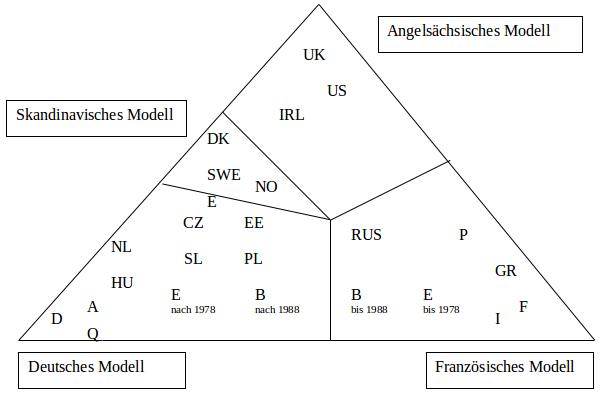
\includegraphics[width=5in]{Material/VerwaltungsModelle}\\
\scriptsize{Quelle: \cite{lipumb05}: 68}
\end{figure}

Aus dem Überblick wird erkennbar, dass es in der EU kein gemeinsames Modell gibt, nach dem eine öffentliche Verwaltung organisiert ist. Vielmehr gibt es nach dieser Darstellung vier Haupttraditionen, die eng mit der historischen Entwicklung in den einzelnen Ländern verbunden sind. Dass die Orientierung in eine bestimmte Richtung nicht statisch ist, zeigen die Beispiele Belgien und England, deren Administrationen zunächst dem französischen Modell angelehnt waren und nun eher dem deutschen Modell folgen, wie im obigen Schema ersichtlich. Weiterhin unterliegen die öffentlichen Verwaltungen Einflüssen, die aus einer generellen Internationalisierung resultieren. So hat das Konzept des „New Public Management“ in allen EU-Mitgliedstaaten zu einem Umdenken und vielfach auch Umbau der Verwaltungen geführt (vgl.\cite{dunhoo}).
\par
Die Modernisierung der öffentlichen Verwaltung ist weltweit in fast allen Ländern zum Thema geworden. In vielen Ländern auf allen Kontinenten sind Aktivitäten zu verzeichnen, deren Ziel eine rationale und effektive Verwaltungsführung ist. Damit verbunden ist meist die Hoffnung auf Kosteneinsparungen, die konsequente Trennung von Verwaltung und Politik, größere Bürgernähe der Verwaltung und/oder verbesserte Aufgabenerfüllung der öffentlichen Hand. Dabei sind mehrere Beweggründe für Verwaltungsmodernisierung zu beobachten:
\par
\begin{itemize}
\item In Ländern mit entwickelten öffentlichen Verwaltungen die Notwendigkeit, Ausgaben im öffentlichen Sektor einzusparen.
\item In Transformationsländern mit nicht existenten Verwaltungsstrukturen oder vormals Kommandowirtschaft die Notwendigkeit, Verwaltungsstrukturen nach modernen Kriterien aufzubauen.
\item Internationale Ausrichtung, z.B. EU-Mitgliedschaft.
\item Globalisierung: Wettbewerb der Länder untereinander bei der Schaffung optimaler Bedingungen für global operierende Unternehmen und Investoren.
\end{itemize}
Man kann zwei Phasen unterscheiden bei dem Austausch von Erfahrungen zwischen Ländern im Feld öffentlicher Verwaltung. Die erste Phase bestand ungefähr von den 1970er Jahren bis Ende des 20. Jahrhunderts. Diese Phase war geprägt von Informalität, Spontaneität und Freiwilligkeit. Kennzeichen war die gegenseitige Beeinflussung der administrativen Systeme, basierend auf Verwaltungsrecht und Gewohnheitsrecht, sowohl in Europa als auch in der Welt. Die zweite Phase des Austausches von Erfahrung und Wissen im Bereich öffentlicher Verwaltung ist seit Beginn des 21. Jahrhunderts auszumachen. Die Überzeugung, dass man die nationalstaatlichen öffentlichen Verwaltungen nicht nur sich selbst überlassen sollte, wurde in der Milleniumserklärung der Vereinten Nationen 2000 in den Blick genommen, die die enge Verzahnung des Kampfes gegen Armut und das Recht auf Entwicklung und „Good Governance“ definierte. 
\subsection{Das Konzept „Good Governance”}
In der vorliegenden Arbeit wird der Begriff „Reform der öffentlichen Verwaltung“ (Englisch: Public Administration Reform, PAR) in einem umfassenden Sinne verstanden; er umfasst den Beamtenapparat, seine rechtliche Verankerung, seine Funktionen, Kompetenzen und Verfahren, unter Einschluss der Verwaltung des Justizsystems. Über den klassischen Begriff der öffentlichen Verwaltung hinaus wird ein umfassenderes Konzept von ‘governance’ zugrunde gelegt. Dieses schließt die Kultur des Regierungshandelns im Sinne der nationalen Entscheidungen hinsichtlich der Ausgestaltung von Staatlichkeit (Legitimität, Effektivität, Transparenz, Pluralität und Verantwortlichkeit) ein, ebenso wie die Beziehungen zwischen Regierung und Parlament.\par
Der Begriff Governance, der zentral ist in der Betrachtung der Verwaltungsmodernisierung in den Ländern, die einen EU-Beitritt anstreben, wird von verschiedenen Institutionen unterschiedlich beschrieben.\par
Die Vereinten Nationen gehen von einer umfassenden Definition von „Governance“ aus, die die Definition einer modernen öffentlichen Verwaltung einschließt. „Governance“ im Gegensatz zum traditionellen Verständnis von „Öffentlicher Verwaltung“ legt einen Schwerpunkt auf Mitgestaltung und Partnerschaft. „Public administration needs to be transformed into a responsive instrument to meet the needs of all citizens“ (\cite{unpan}).\par
Das gewachsene Interesse an einer Governance-Orientierung der Vereinten Nationen wird auf folgende Entwicklungen zurückgeführt:
\begin{itemize}
\item den Erfolg der Marktwirtschaft und das Scheitern der Planwirtschaft;
\item die Tendenz, demokratische Regierungsformen mit wirtschaftlichem Erfolg gleichzusetzen;
\item die weltweite Krise der öffentlichen Finanzen, die in vielen Staaten die Frage nach der Rolle und der Effizienz des Staates neu gestellt hat; 
\item die gestiegene Wahrnehmung und Verärgerung über Korruption in Regierung und Verwaltung;
den Zusammenbruch der ehemaligen Sowjetunion und die ethnischen Konflikte auf dem Balkan und in Afrika, die die neuen Staaten vor große Umbauaufgaben auch ihres politischen Systems stellen (vgl. \cite{undp}: 18).
\end{itemize}
Die Weltbank beschreibt das Konzept als “the traditions and institutions by which authority in a country is exercised for the common good” (\cite{weltbank}: 1). Die sechs Governance-Indikatoren der Weltbank gelten mittlerweile als Standardkriterien zur Bewertung von Good Governance: 
\begin{itemize}
\item Politische Mitspracherechte (Voice and Accountability),
\item Politische Stabilität und Gewaltkontrolle (Political Stability and No Violence);
\item Effektivität des Regierens (Government Effectiveness),
\item Qualität regulativer Politik (Regulatory Quality),
\item Rechtsstaatlichkeit (Rule of Law),
\item Korruptionskontrolle (Control of Corruption) (vgl. \cite{kaufmann}).
\end{itemize}
Im Laufe der 1990er Jahre übernahmen auch die in der OECD zusammengeschlossenen Geber sowie die EU das Konzept der „guten Regierungsführung“.\par
Die SIGMA-Initiative der OECD versucht in ihrer Veröffentlichung zu ‘European Principles of Public Administration’ im Jahr 1999, ebenfalls an den Weltbankindikatoren angelehnt, Prinzipien für die öffentlichen Verwaltungen in ihren Mitgliedstaaten aufzustellen. Folgende Indikatoren werden genannt: 
\begin{itemize}
\item reliability and predictability (legal certainty or judicial security); 
\item openness and transparency; 
\item accountability; 
\item efficiency and effectiveness (vgl. \cite{oecd99}: 8ff).
\end{itemize}
An dem Good-Governance-Verständnis von Weltbank und IWF sowie OECD orientiert sich auch die Europäische Union. Die Europäische Kommission hat im Jahr 2001 ihr Weißbuch „Europäisches Regieren“ veröffentlicht, das ebenfalls Kriterien guter Regierungsführung enthält (vgl. \cite{czada2010}). Dort werden folgende Prinzipien als Merkmale von Good Governance definiert:
\begin{itemize}
\item Transparenz: Institutionen sollten in ihrem Handeln transparent sein und erklären, wie ihre Entscheidungen zustande kommen.
\item Partizipation: Die Qualität und Effektivität von Politik hängt wesentlich von umfassender Partizipation ab.
\item Übernahme von Verantwortung: Institutionen müssen erklären, warum sie etwas tun, und auch dafür Verantwortung übernehmen.
\item Effektivität: Policies müssen effektiv und zeitnah umgesetzt werden mit dem Ziel, das Benötigte auf der Basis von definierten Zielen zu liefern.
\item Kohärenz: Policies und Handlungen müssen kohärent und nachvollziehbar sein.
(vgl. \cite{euko01}: 13).
\end{itemize}
Gute Regierungsführung ist demnach im Wesentlichen gleichbedeutend mit einer leistungsfähigen, berechenbaren und transparenten staatlichen Verwaltung. Sie setzt „ein funktionierendes öffentliches Buchführungs- und Rechnungswesen ebenso voraus wie einen verbindlichen rechtlichen Rahmen, der privatwirtschaftlichen Wettbewerb ermöglicht“ (\cite{schmitz09}: 132).
\par
In der Debatte um die Notwendigkeit stabiler Institutionen und einer effektiven öffentlichen Verwaltung schwingt explizit oder implizit mit, dass die Modernisierung der öffentlichen Verwaltung die Demokratisierung vorantreibt. „Die Demokratie ist heute eigentlich keine Volksregierung, sondern eine Volksverwaltung – die Administration ist die eigentliche Aufgabe der Demokratie“ (Masaryk, zit. nach \cite{czerwick}: 14). Czerwick merkt dazu an, dass in der wissenschaftlichen Literatur davon ausgegangen wird, dass demokratische Systeme nur überleben können, wenn sichergestellt ist, dass die öffentlichen Verwaltungen ein Mindestmaß an struktureller Übereinstimmung mit demokratischen Normen, Institutionen und Prinzipien aufweisen.
\par
Vor diesem Hintergrund ist im Zusammenhang mit der (weiteren) Demokratisierung der Staaten des Westlichen Balkans und ihrem Wunsch einer Aufnahme in die Europäische Gemeinschaft die Frage nach dem Status quo der Verwaltung in diesen Ländern unumgänglich. Es wird deutlich, dass die öffentliche Verwaltung ein zentrales Element ist für die weitere Entwicklung, Demokratisierung und ultimativ den EU-Beitritt der Balkanstaaten. Dennoch ist dieser Zusammenhang von der Forschung bislang wenig beachtet worden. Die vorliegende Arbeit versucht erste Schritte, um diese bemerkenswert große Forschungslücke zu schließen. In Anbetracht der kaum vorhandenen Literatur wird das Thema Verwaltungsmodernisierung im Westbalkan im Kontext der EU-Erweiterung in der vorliegenden Arbeit von mehreren Seiten betrachtet. Die historische Perspektive fließt mit ein, in der Hoffnung auch aus dieser Betrachtung Hinweise zur Beantwortung der Forschungsfragen zu erhalten.
\section{Methodisches Konzept}
In der vorliegenden Arbeit wird eine Annäherung an ein bisher weitgehend nicht untersuchtes Thema, die Bedeutung der Reform der öffentlichen Verwaltung im Westlichen Balkan im Kontext der EU-Erweiterung, vorgenommen. Da mit dieser Untersuchung quasi Neuland betreten wird, wurde eine Methode gewählt, die es ermöglicht, das Thema von unterschiedlichen Seiten aus zu betrachten. Gewählt wurde ein kaleidoskopisches Verfahren, mittels dessen versucht wird, Antworten auf die zentrale Frage und die weiterführenden Fragen der Untersuchung finden. Die Vorgehensweise in der vorliegenden Arbeit ist im Rahmen des Forschungsansatzes der Triangulation verortet. Triangulation findet vor allem in der empirischen Sozialforschung Anwendung. Mit unterschiedlichen Methoden oder Sichtweisen, bzw. Daten wird versucht ein Phänomen zu erklären. Ursprünglich kommt der Begriff Triangulation aus der Landvermessung, wo er folgendermaßen verwendet wird:\par
„Triangulation is the method of location of a point from two others of known distance apart, given the angles of the triangle formed by three points. By repeated application of the principle, if a series of points form the apices of a chain or network of connected triangles of which the angles are measured, the lengths of all the unknown sides and the relative positions of the points may be computed when the length of one of the sides is known” (\cite{clark}: 145).\par
In der sozialwissenschaftlichen Forschung wurde die Triangulation als Methode entwickelt, um von verschiedenen Referenzpunkten aus die Position des (Forschungs-)Objektes zu lokalisieren (vgl. Smith 1975, zit. nach \cite{jick}: 136). Auf dieser Grundlage definiert Flick: „Triangulation beinhaltet die Einnahme verschiedener Perspektiven auf einen untersuchten Gegenstand oder allgemeiner: bei der Beantwortung von Forschungsfragen. Diese Perspektiven können sich in unterschiedlichen Methoden, die angewendet werden, und/oder unterschiedlichen gewählten theoretischen Zugängen konkretisieren, wobei beides wiederum miteinander in Zusammenhang steht bzw. verknüpft werden sollte. Weiterhin bezieht sie sich auf die Kombination unterschiedlicher Datensorten jeweils vor dem Hintergrund der auf die Daten jeweils eingenommenen theoretischen Perspektiven“ (\cite{flick08}:12).\par

In ähnlicher Weise resümiert Schirmer: „Triangulation meint – allgemein gesprochen – die Betrachtung eines ‚Punktes’ aus mehreren Perspektiven mit dem Ziel, diesen Punkt umfassender oder vollständiger zu verstehen, sozusagen ein kompletteres Bild zu entwerfen; damit sollen gleichzeitig Verzerrungen oder Fehlblicke vermieden oder relativiert werden, die Resultat einer bestimmten Perspektive sind.“ (\cite{schirmer}: 100). \par
Der Kern der Triangulation als Methode in der sozialwissenschaftlichen Forschung ist die Kontrastierung. In der vorliegenden Arbeit werden die Erkenntnisse aus der Literaturanalyse anhand von Interviews mit Experten überprüft und so eine Kontrastierung vollzogen, die möglicherweise zu neuen Erkenntnissen und weiterführenden Fragestellungen führt. Diese Vorgehensweise erscheint als eine gute Grundlage für weitergehende Forschung zu dem bisher wenig beleuchteten Thema dieser Arbeit.\par

In der praktischen Anwendung kann man zwei unterschiedliche Lesarten zu Triangulation feststellen. Im ersten Fall wird die Triangulation als Validierung von Forschungsergebnissen durch die Verwendung unterschiedlicher Methoden gesehen. Eine andere Lesart ist die Triangulation mit dem Ziel, ein umfassenderes Bild des Gegenstandsbereichs zu erzielen und den Untersuchungsgegenstand von unterschiedlichen Perspektiven her zu betrachten (vgl. \cite{kelle}: 50). Für die vorliegende Untersuchung wird die Triangulation im letzteren Sinne verwandt.
\par
Es wird versucht, über eine Betrachtung der historischen Verwaltungstradition und Verwaltungsentwicklung in drei benachbarten Ländern des Westlichen Balkans (Albanien, Mazedonien und Montenegro) Gemeinsamkeiten und Unterschiede aufzuspüren, die für den Status quo der Verwaltungsentwicklung in den Ländern relevant sein könnten.\par
Der aktuelle Bezugspunkt der Untersuchung und allen drei Untersuchungsländern gemein ist die Aufnahmeperspektive in die EU. Neben der Entwicklung der Beziehungen der Untersuchungsländer zur EU wird daher auch die Unterstützung der EU im Rahmen der Heranführungshilfe für die Aufnahmekandidaten beschrieben.\par
In einem weiteren Teil der Arbeit werden von der Verfasserin durchgeführte Experteninterviews zu den Forschungsfragen der Arbeit ausgewertet. Die Interviews betreffen thematisch den Status quo der Verwaltungsmodernisierung in den Untersuchungsländern und die Unterstützung durch die EU. Sechs Interviews wurden hierzu mit hochrangigen Beamten der EU und OECD / SIGMAs durchgeführt. Um die Perspektive in den Untersuchungsländern zu erfassen, wurden außerdem in jedem der drei Länder jeweils ein Vertreter der Regierung und ein Vertreter einer Nichtregierungsorganisation (NRO/NGO) interviewt. Alle Interviewpartner waren intensiv mit Verwaltungsmodernisierung befasst und sind in diesem Sinne Experten zum Thema. Insgesamt wurden also zwölf Interviews durchgeführt, die für die vorliegende Arbeit ausgewertet wurden.
\par
In Anbetracht der noch sehr überschaubaren Literatur zum Prozess der Verwaltungsmodernisierung in den Westbalkanländern unter dem Einfluss des EU-Erweiterungsprozesses stellt die Auswertung der Experteninterviews einen unverzichtbaren Beitrag dar. Dabei geht es nicht vorrangig um die Validierung von Ergebnissen der Literaturdurchsicht, sondern um eine Erweiterung der Forschungsperspektive unter Einschluss der persönlichen Erfahrungen und Meinungen von Experten, die sich mit dem Thema in der täglichen Berufspraxis beschäftigten.\par
In die vorliegende Untersuchung fließen ferner Eindrücke aus der eigenen beruflichen Praxis ein. Die Verfasserin hat mehrere Jahre für die OSZE in Südosteuropa im Bereich Demokratisierung vor allem in der Durchführung und Beobachtung von Wahlen gearbeitet (Kosovo noch unter internationaler Administration, Bosnien-Herzegowina, Albanien und Montenegro). Ein wiederkehrender Befund durchzieht diese jahrelange Beschäftigung. Einerseits handelt es sich bei dieser Region geografisch um Europa. Im gemeinsamen Land Jugoslawien bestanden über viele Jahre politisch und ökonomisch enge Kontakte mit den Ländern der EU und der EU als Institution. Andererseits erscheint die Region heute weit von Europa entfernt. So findet Berichterstattung in den westeuropäischen Medien kaum statt. Dieses mangelnde Interesse kann nur zum Teil mit den Kriegen Anfang der 90er Jahre erklärt werden, die zu ökonomischen und politischen Rückschritten führten.\par
Der Widerspruch zwischen einerseits geografischer Zugehörigkeit zu Europa und andererseits wahrnehmbar großer Entfernung zu Westeuropa spiegelt sich auch in der Herangehensweise der EU gegenüber der Region. Einerseits hat die EU den Staaten des Westbalkans seit 2003 einen Beitritt zur EU in Aussicht gestellt. Andererseits sind Auflagen seitens der EU formuliert worden, die in wesentlichen Punkten über die Anforderungen der früheren Aufnahmewellen hinausgehen. Auch wird die bisher gängige Praxis einer gemeinsamen EU-Aufnahme mehrerer Staaten für die Länder des Westbalkans ausgeschlossen.
\section{Aufbau der Arbeit }
Übergeordneter Bezugsrahmen für die vorliegende Arbeit ist zunächst die Konditionalität der EU, die derzeit den theoretischen Hauptstrang der Europäisierungsforschung darstellt. Das Konzept der Konditionalität wird im zweiten Kapitel aus der Demokratisierungs- und Transformationsforschung hergeleitet und bildet den ersten Rahmen der Untersuchung.
Ebenfalls im zweiten Kapitel wird der Prozess der EU-Erweiterung in der Praxis dargestellt. Dabei wird auch ausführlich auf den Stellenwert der Verwaltungsmodernisierung in diesem Prozess eingegangen. Hierbei ist zentral, dass Verwaltungsentwicklung im Erweiterungsprogramm der EU nicht explizit vorkommt. Eine implizite Bezugnahme ist dennoch erkennbar mit dem Konzept des Europäischen Verwaltungsraums, das ebenfalls dargestellt wird. Für dieses Kapitel werden Veröffentlichungen der EU und anderer internationaler Akteure (OECD/SIGMA, UNDP, Weltbank usw.) hinsichtlich des Stellenwertes von Verwaltungsentwicklung innerhalb des Erweiterungsprozesses ausgewertet. Ein wichtiger Teilaspekt der Betrachtung in diesem Kapitel ist die Auswertung der letzten Aufnahmewelle der EU hinsichtlich der Erfahrungen mit und der Nachhaltigkeit von Verwaltungsmodernisierung. Abschließend werden im zweiten Kapitel die Hilfen der EU für die Verwaltungsentwicklung in Kandidatenländern vorgestellt. \par
Die Ausgangslage auf dem Westbalkan ist Gegenstand des dritten Kapitels und bildet einen weiteren Rahmen für die Arbeit. Es wird auf die sozialistische (Jugoslawien) und kommunistische (Albanien) Verwaltungsgeschichte ebenso eingegangen wie auf die zeitlich davor gelagerten imperialen Einflüsse auf die Verwaltung (Österreich-Ungarn, Osmanisches Reich). Dieser Teil der Arbeit wird vorwiegend mittels einer Literatur-Auswertung durchgeführt. Auch die Sichtung von Akten der Österreichischen Militärverwaltung in Montenegro und Albanien während des Ersten Weltkrieges durch die Autorin im Staatsarchiv in Wien fließt in diesen Teil der Untersuchung ein. Als Bezugsrahmen dieses Teiles der Arbeit dient der Legacy-Ansatz, der auch für die vergleichende Verwaltungsforschung anwendbar ist. An die historische Betrachtung schließt sich die kursorische Darstellung der Verwaltungsentwicklung in den drei Untersuchungsländern in der Demokratie an.
\par
Der empirische Teil der Arbeit folgt im vierten Kapitel, bestehend aus zwölf Experteninterviews. Im ersten Teil dieses Kapitels wird die angewandte Methode für die Durchführung der Experteninterviews dargestellt, einschließlich des Vorgehens bei der Auswertung. Im Hauptteil des vierten Kapitels werden die Ergebnisse der Experteninterviews analog der behandelten Themenstränge dargestellt und analysiert.\par
Das Gesamtergebnis der Untersuchung wird im fünften Kapitel zusammengefasst dargestellt.